As we found in \autoref{section: TOV equation}, the Tolman-Oppenheimer-Volkoff equation, \autoref{TOV}, determines the pressure as a function of the radius of a star given the equation of state and the central pressure.
From \autoref{chapter: thermodynamics}, we have various equations of state for the pion condensate.
In this chapter, we will apply these results to study pion stars, bosonic stars composed of a gravitationally bound pion condensate, first proposed by \citeauthor{brandtNewClassCompact2018}~\autocite{brandtNewClassCompact2018}.



\section{Units and limiting radius}

We can gain some insights by reviewing the characteristic quantities of the problem.
The characteristic mass and length, as discussed in \autoref{section: TOV equation}, are found by setting $k_1 = k_2 = k_3 = 1$.
These are the dimensionless constants of the TOV equation, \autoref{dimensionless constants TOV}.
At leading order, the bare constants $f$ and $\bar m$ are related to physical constants by $f = f_\pi$ and $m = m_\pi$, the pion decay constant and the pion mass.
Using the values for $f_\pi$ and $m_\pi$ as given in \autoref{section: units} and reinstating $c$ and $\hbar$, these quantities are given by
%
\begin{align}
    u_0 & =m_\pi^2 f_\pi^2 \frac{c}{\hbar^3}
    = 3.216\cdot 10^{33} \, \text{J}\,\text{m}^{-3}, \\
    m_0 & = \frac{c^4}{\sqrt{\frac{4 \pi}{ 3} u_0 G^3}} = 64.21\, M_\odot, \\
    r_0 & = \frac{G}{c^2} m_0 = 94.79 \, \text{km}.
\end{align}
%
We, therefore, expect both the radius and mass of the pion star to be around one order of magnitude larger than the star made up of cold neutrons.
\todo[inline]{Can we make a better argument by setting gravitational + internal energy equal 0?}


In \autoref{section: thermodynamics leading order}, we found that the leading order, the non-relativistic limit of the equation of state of a pure pion-condensate, without electromagnetic interaction, is $\tilde p =8^{-1} \tilde u^2$.
That is, it is a polytrope with $\gamma = 2$.
As discussed in \autoref{subsection: Newtonian limit and polytropes}, this corresponds to a situation where the radius of the star is independent of the central pressure, at least in the Newtonian limit of gravity.
When simulating the Newtonian, non-relativistic limit of the pion star, we should expect the radius to be constant.
From \autoref{Radius polytrope}, the radius is $R = C \xi_1$, where
%
\begin{equation}
    C = \frac{1}{\sqrt{4(4\pi ) G u_0}} = \frac{1}{\sqrt{12}}r_0,
\end{equation}
%
and $\xi_1$ is the root of the Lane-Emden function $\theta(\xi)$ for polytrope index $n=1$, the solution to
%
\begin{equation}
    \theta'' + \frac{2}{\xi} \theta' + \theta = 0.
\end{equation}
%
By substituting $\theta$ for its power series expansion, $\theta = \sum_n a_n \xi^n$, we get
%
\begin{equation}
    \sum_n \left[ (n+2)(n+1) a_{n+2} + 2(n+1) a_{n+1} \xi^{-1} + a_n \right] \xi^n = 0.
\end{equation}
%
This must be obeyed for arbitrary $\xi$.
We therefore get the recursion relation $a_{n+2} = - a_n / (n+1)(n+2)$.
With our boundary condition, the solution is
%
\begin{equation}
    \theta(\xi) = \frac{\sin(\xi)}{\xi},
\end{equation}
%
and the first root is therefore $\xi_1 = \pi$.
With this, we get a closed-form expression for the stellar radius of this non-relativistic and Newtonian limit---which we expect the full theory to approach as the central pressure decreases---namely
%
\begin{equation}
    \label{radius pion star nr limit}
    R = \frac{\pi}{\sqrt{12}} r_0 = 85.97 \, \text{km}.
\end{equation}
%
When including electromagnetic interactions, as done in \autoref{subsection: including electromagnetism lo eos}, the non-relativistic equation of state remains a polytrope with $\gamma=2$, however with a new constant by a factor $(1+\Delta)^2$, where $\Delta = \Delta m^2_\text{EM}/m_\pi^2$.
This affects the maximum radius, which now is
%
\begin{equation}
    \label{maximum mass pion star with em interaction}
    R = \frac{\pi}{\sqrt{12}(1 + \Delta)} r_0 = 80.40 \, \text{km}.
\end{equation}
%
These limits are only available when considering the pion condensate alone, without leptons.
As we found, the inclusion of leptons will change the low-density limit of the equation of state, and it is only for $\gamma=2$ where the Lane-Emden equation admits a non-zero limit radius of this sort.


\section{Numerical results}


\todo[inline]{Pass på at tall i tekst matcher med figurer!}
In this section, we present the results of integrating the TOV-equation numerically.
The computer code used to obtain these results is discussed in \autoref{appendix: code}.

\subsection{Pion star of pure pion condensate}


We start with the simplest case of a pure pion condensate, in which there are only strong interactions, to leading order as described in \autoref{subsection: pure pion condensate}.
The equation of state of this system is shown in \autoref{fig: equation of state pions}.

\autoref{fig: pressure and mass for pion star} show the pressure and mass as a function of radius for varying values of central pressure.
The quantities are normalized to the stellar radius, stellar mass, and central pressure, respectively.
The black dashed line corresponds to the configuration with the maximum mass.
We see that both the pressure and mass distribution are very similar for stars with a mass less than the maximum.
As the central pressure increase beyond that of the star with maximum mass, the pressure gradient close to the center grows sharply.
This is similar to what we saw in the case of an incompressible fluid, \autoref{subsection: incompressible fluid}.

\autoref{fig: mass-radius relation pion star} shows the mass-radius relation for the pion star.
As in the case of the neutron star, it has a maximum mass, in this case of $M_\text{max} = 10.47\, M_\odot$.
However, in contrast to the case of the neutron star, the stellar radius approaches a maximum radius as the central pressure decreases.
This matches our expectation from the non-relativistic, Newtonian limit.
We see that the largest radius in our results, corresponding to  $p_c = 10^{-6} \, p_0$, is $R = 85.82 \, \text{km}$, which is in good agreement with our earlier analysis, \autoref{radius pion star nr limit}.

\autoref{fig: mass-radius relation pion star comparison} compares the mass-radius relation from the full equation of state and TOV equation with various limits.
In the non-relativistic, Newtonian limit, the stellar radius is independent of the mass, as we found in our earlier analysis.


\begin{figure}[!htb]
    \centering
    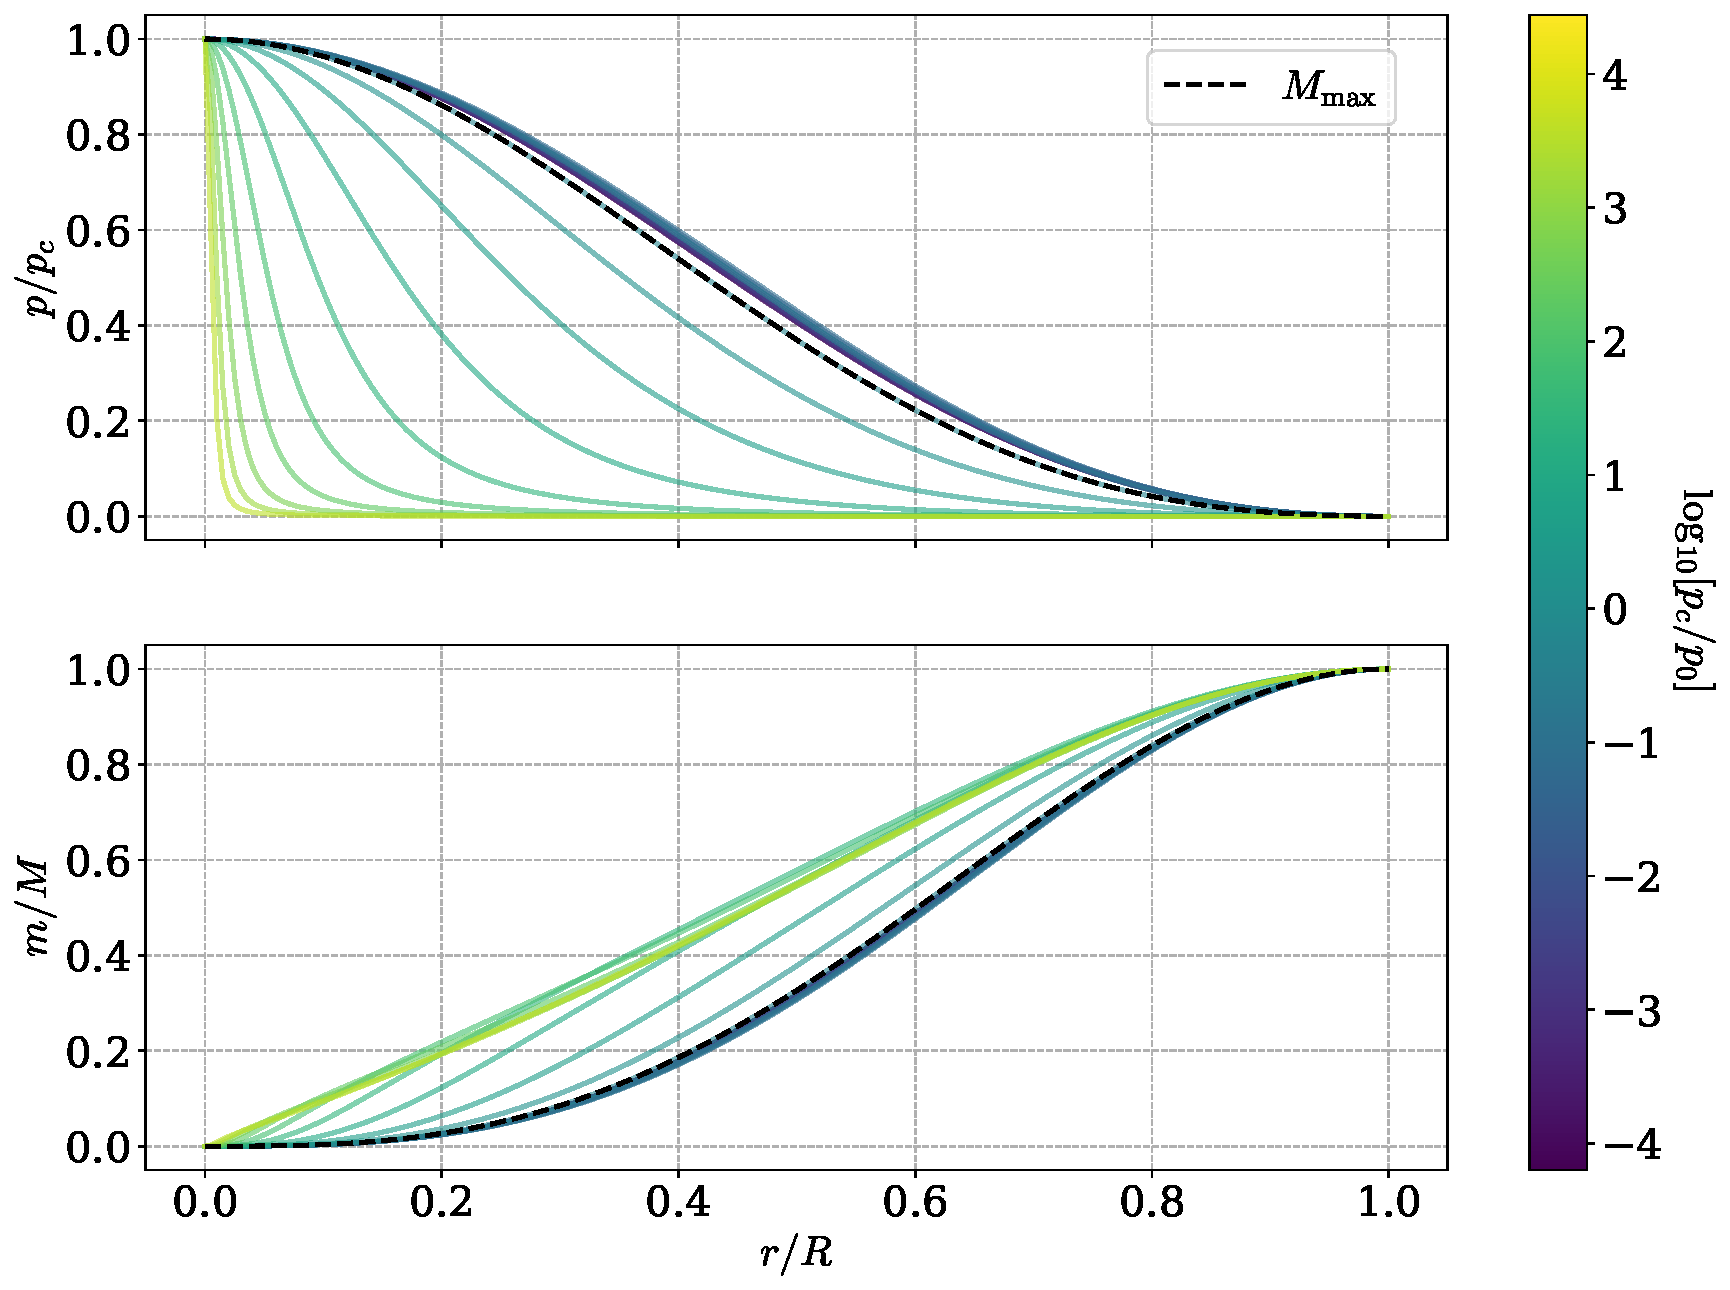
\includegraphics[width=0.8\textwidth]{../scripts/figurer/pion_star/pressure_mass_pion_star.pdf}
    \caption{
    Top: The pressure normalized to the central pressure, as a function of radius, normalized to the stellar radius.
    Bottom: The mass, normalized to the stellar mass, within a radius $r$, normalized to the stellar radius.
    Both plots show a range of stars with different central pressures, indicated by the color.
    The black dashed line corresponds to the star with the largest mass.
    }
    \label{fig: pressure and mass for pion star}
\end{figure}

\begin{figure}[!htb]
    \centering
    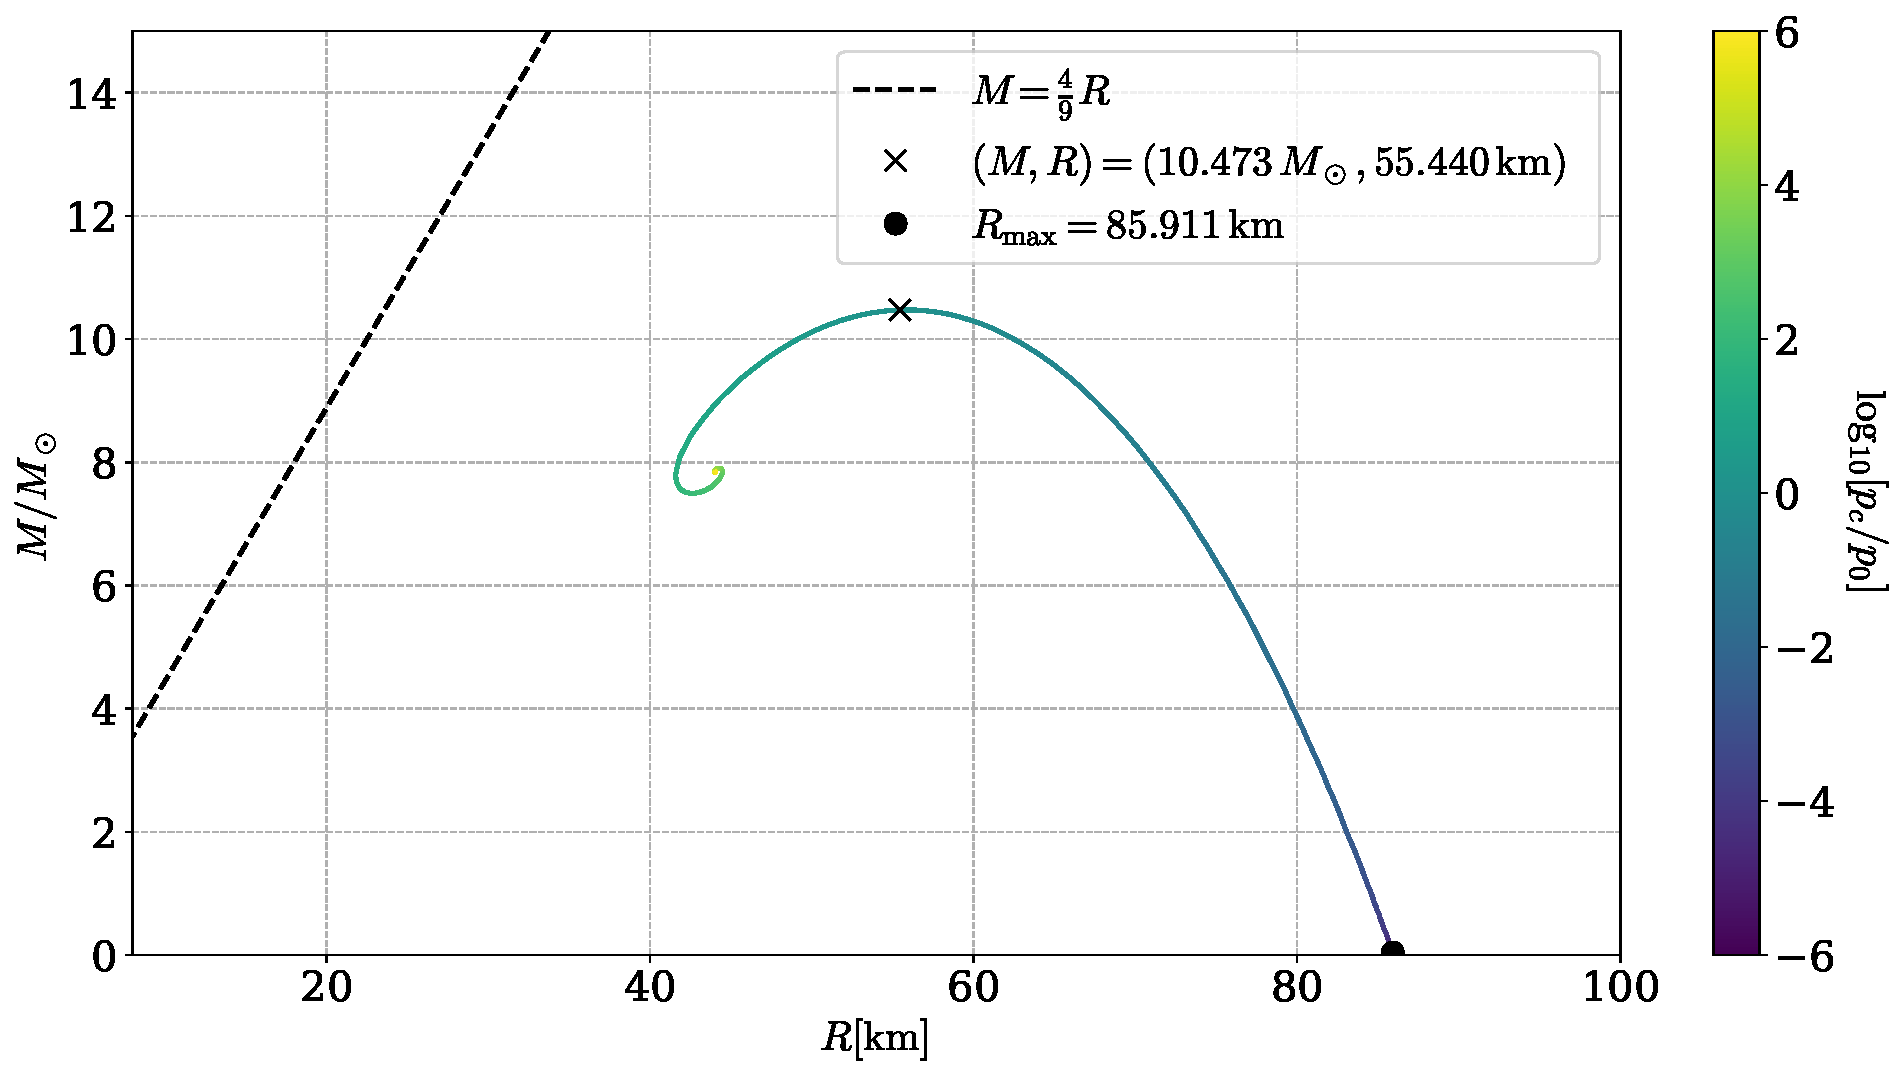
\includegraphics[width=0.85\textwidth]{../scripts/figurer/pion_star/mass_radius_pion_star.pdf}
    \caption{
        The lowest order mass-radius relation of a pion star using two-flavor chiral perturbation theory.
        The mass is given in units of solar masses, while the radius is measured in kilometers.
        This line is parameterized by the central pressure $p_c$ of the star, as indicated by the color gradient.
        The dashed black line indicates the theoretical maximum mass for a given radius, and any configuration above it will collapse to form a black hole.
        }
        \label{fig: mass-radius relation pion star}
\end{figure}

\begin{figure}[!htb]
    \centering
    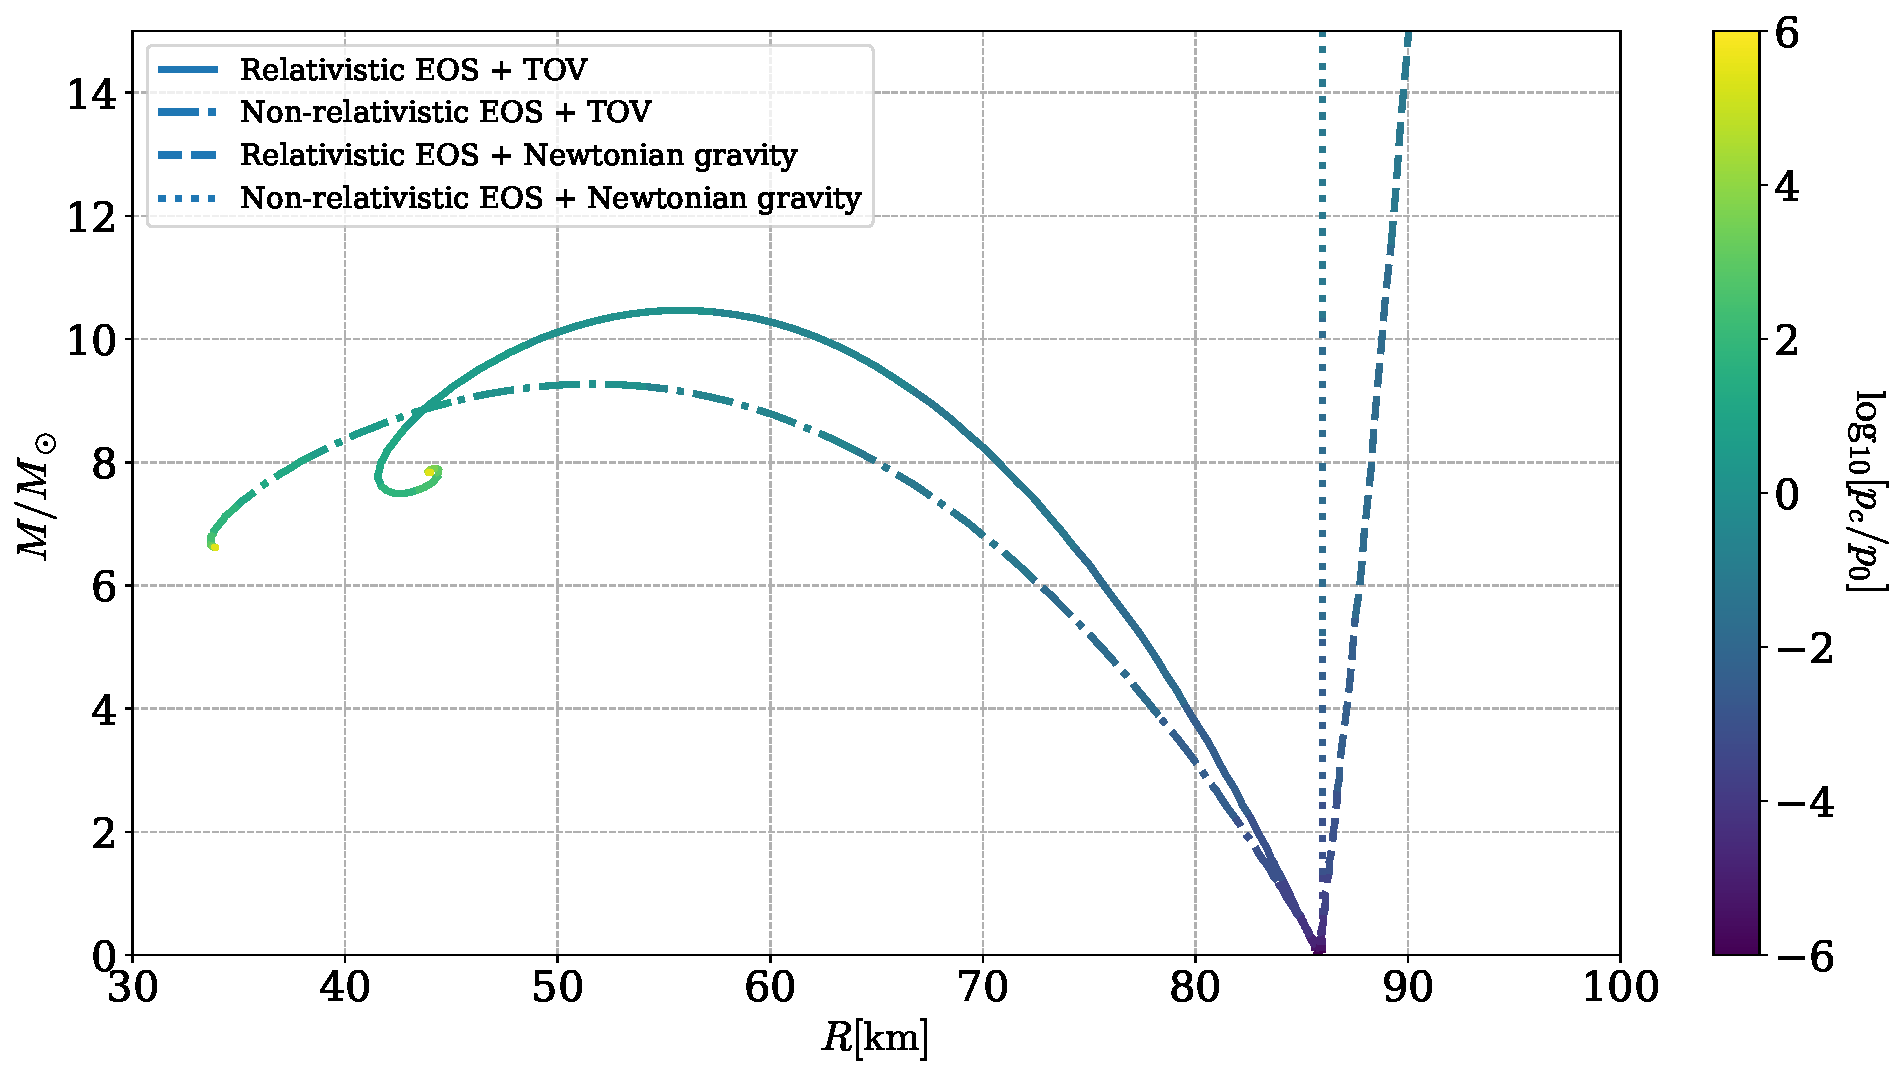
\includegraphics[width=0.85\textwidth]{../scripts/figurer/pion_star/mass_radius_comparison.pdf}
    \caption{
        The mass-radius relationship of the pion star from the full, leading-order equation of state from two-flavor chiral perturbation and the TOV equation, compared with results in various limits.
        }
        \label{fig: mass-radius relation pion star comparison}
\end{figure}



\FloatBarrier
\subsection{Including electromagnetic contributions}

As we found in \autoref{subsection: including electromagnetism lo eos}, the electromagnetic interaction of the pseudoscalar mesons contributes to the equation of state, even at leading order.
\autoref{fig: pressure and energy with EM interaction} shows the pressure and energy density, normalized to their characteristic quantities, as a function of chemical potential above the critical value, normalized to $\bar m$.
\autoref{fig: eos chpt em interaction} shows the equation of state.
The results with and without electromagnetic results are compared.
We see that the inclusion of electromagnetic contributions results in a less stiff equation of state; a given pressure corresponds to a higher energy density when including electromagnetic interactions.

\autoref{fig: mass-radius relation leading order pion star with em interaction} shows the mass-radius reaction of the pion star when the electromagnetic interaction is taken into account.
We see that the shape of the curve has not changed much from our earlier result. 
Both the maximum mass and radius are slightly smaller.
The new result for maximum radius, $R_\text{max} = 80.35 \, \text{km}$, is in excellent agreement with our expectation, \autoref{maximum mass pion star with em interaction}.
The result with and without electromagnetic interaction is compared in \autoref{fig: mass-radius relation comparison}.
As discussed in \autoref{section: cold fermi star}, we expect a stiffer equation of state to correspond to a more massive star, as happens in this case.

\begin{figure}[!htb]
    \centering
    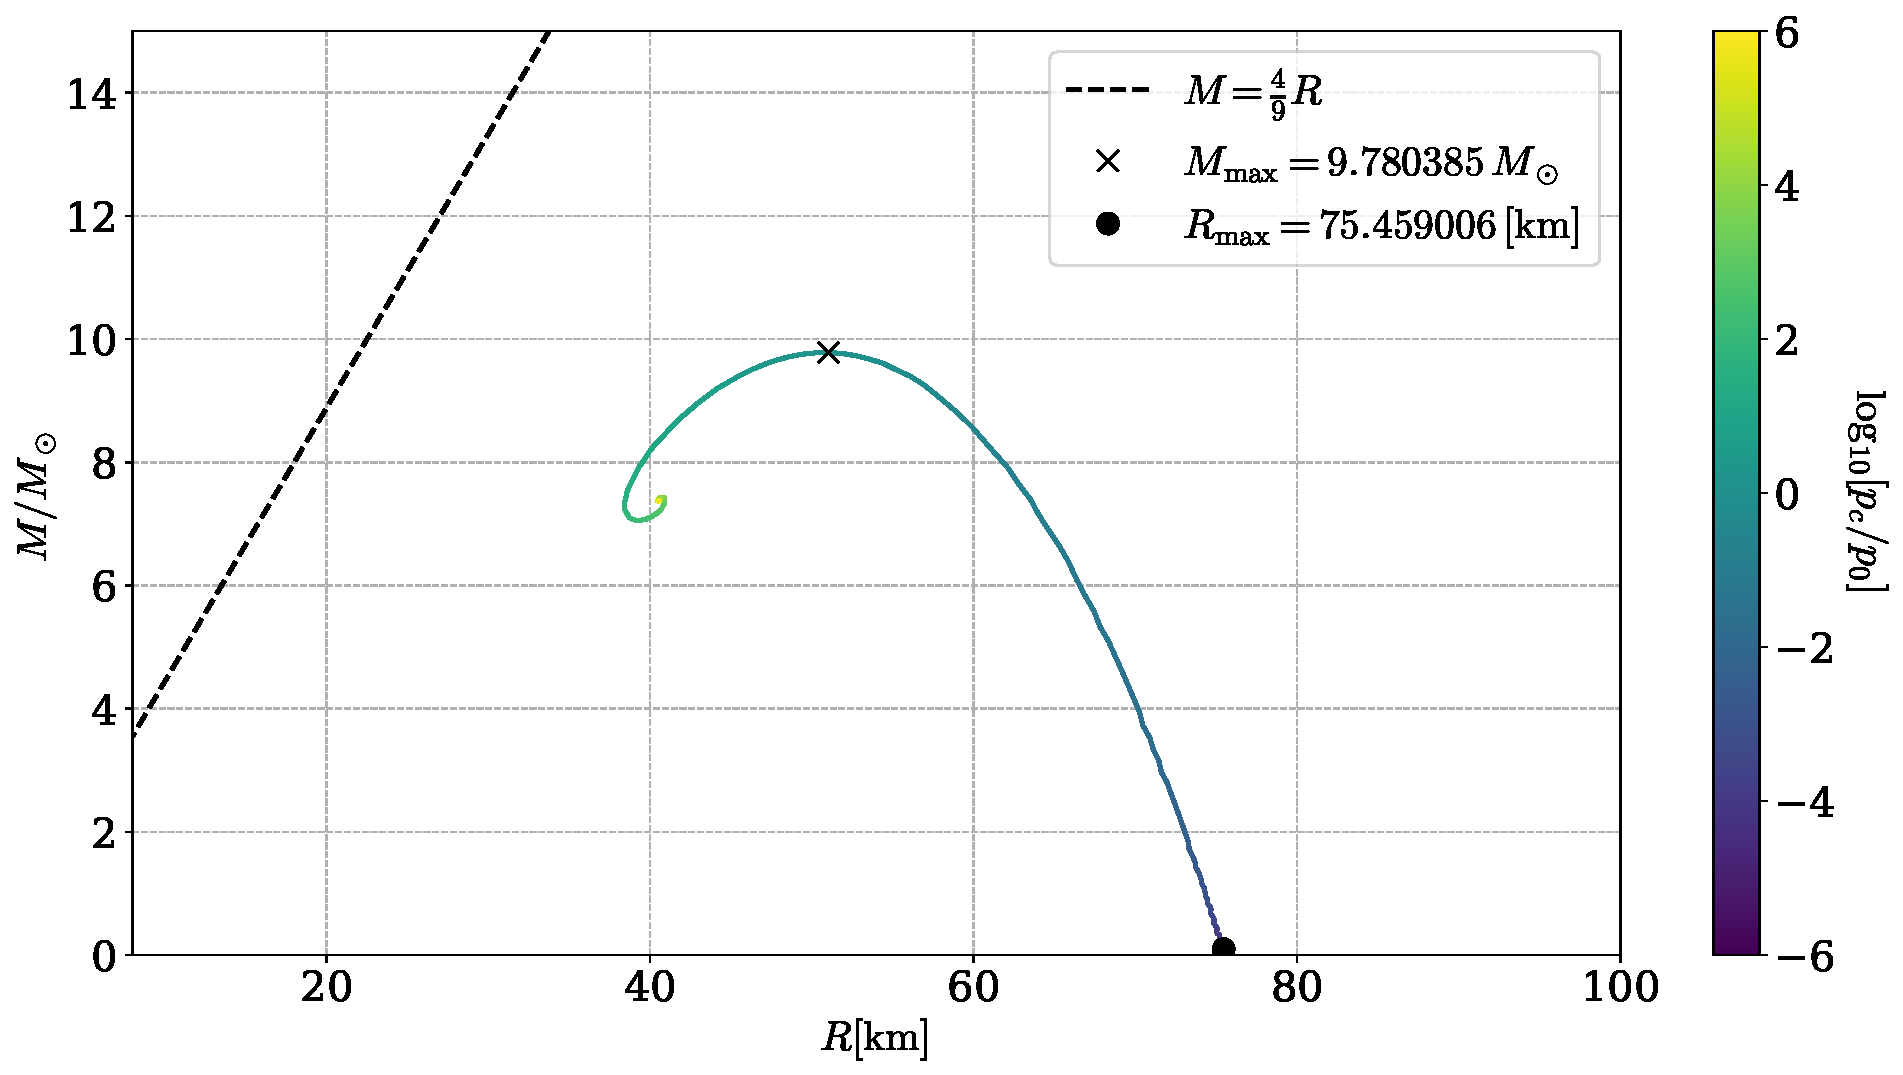
\includegraphics[width=0.85\textwidth]{../scripts/figurer/pion_star/mass_radius_pion_star_EM.pdf}
    \caption{
        The mass-radius relation of a pion star including electromagnetic interactions, parameterized by the logarithm of the central pressure.
        The dashed line shows the absolute limiting mass for a given radius.
        The cross indicates the maximum mass configuration, and the dot the maximum radius configuration.
        The mass is given in units of solar masses, while the radius is in kilometers.
        }
    \label{fig: mass-radius relation leading order pion star with em interaction}
\end{figure}


\begin{figure}[!htb]
    \centering
    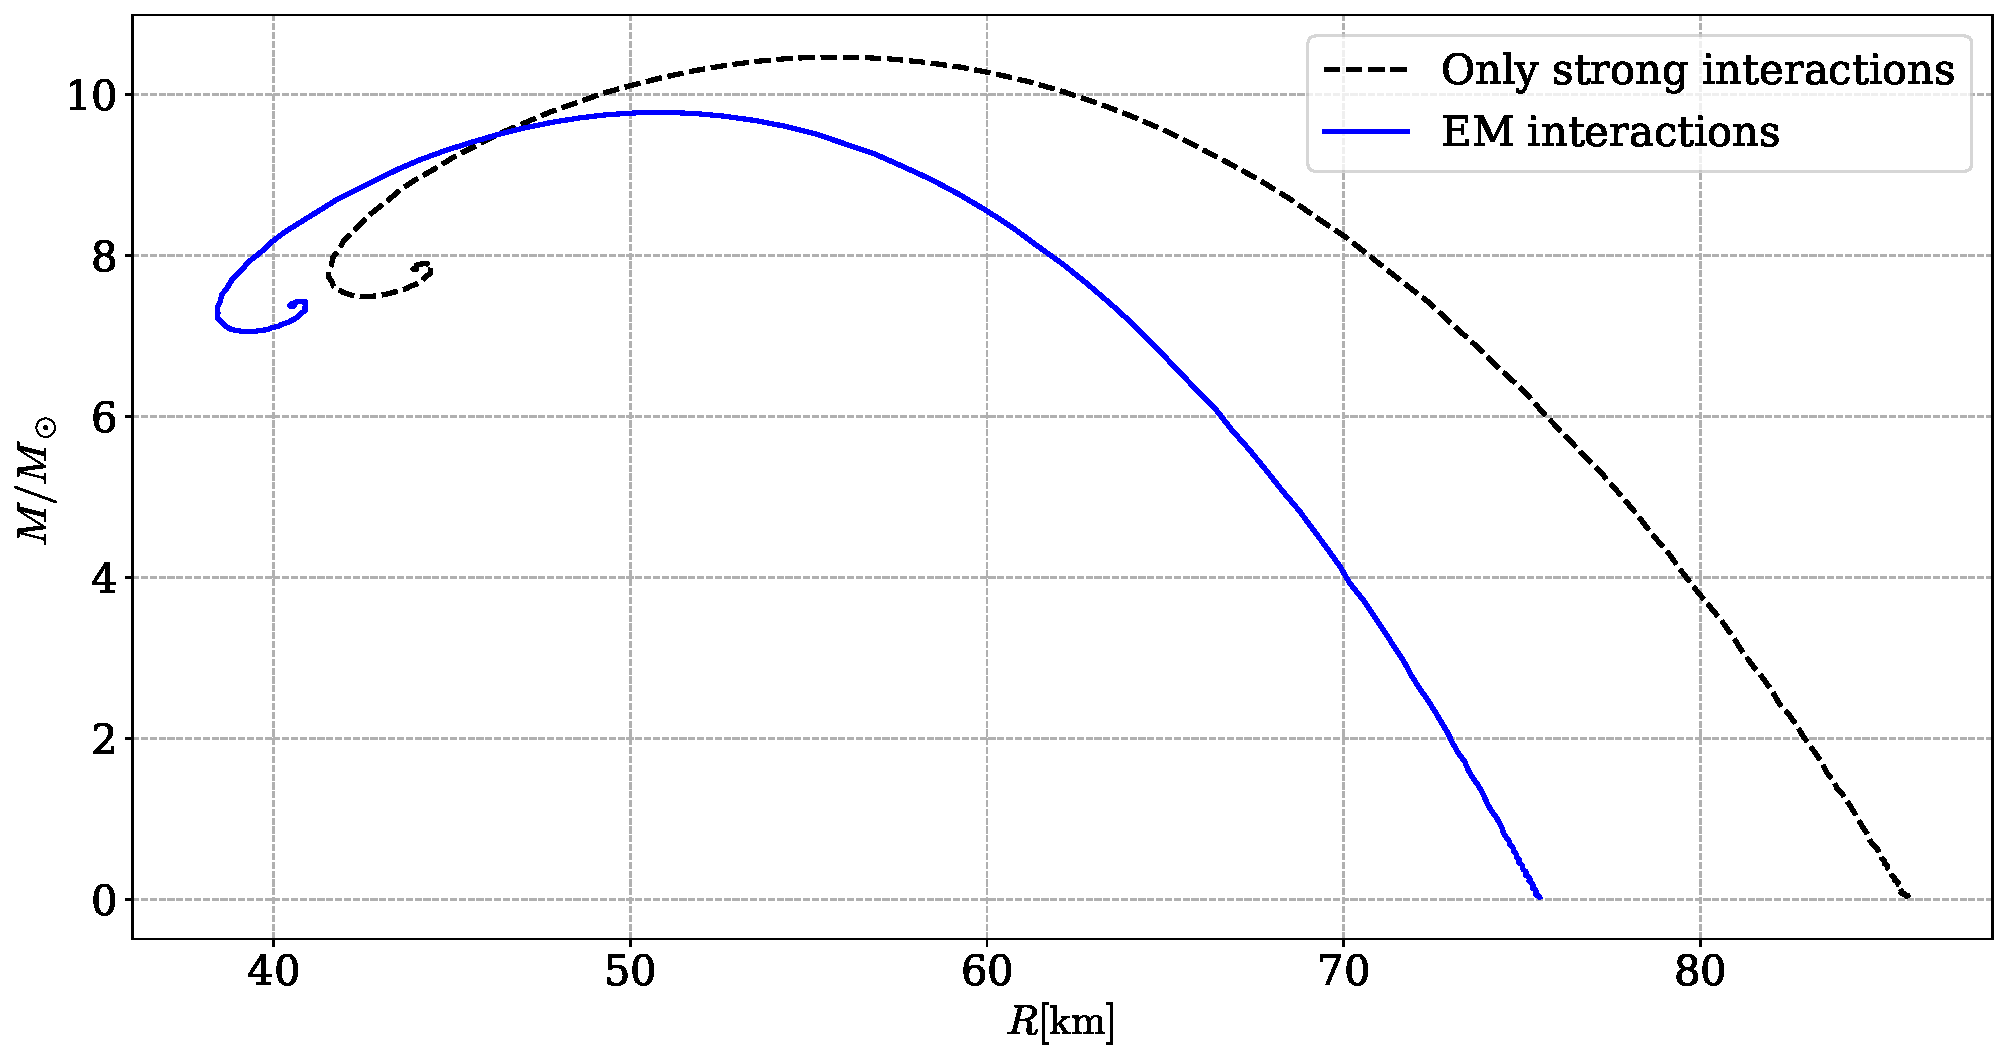
\includegraphics[width=0.8\textwidth]{../scripts/figurer/pion_star/mass_radius_pion_star_compare.pdf}
    \caption{
        The mass-radius relation of pion stars with and without the effects of electromagnetism included.
        The radius is given in kilometers and the mass in units of the solar mass.
        The marked points are the maximum mass and corresponding radius of the stars.
        }
        \label{fig: mass-radius relation comparison}
\end{figure}



\FloatBarrier
\subsection{Charge neutral stars}


We now apply the results from \autoref{section: charge neturality}, where we added a lepton to enforce charge neutrality.
As the electromagnetic force is long-range, we should expect any macroscopic astronomical object to be charge neutral.
First, we apply the system of pions and one charged lepton.
The star with electrons is shown in \autoref{fig: mass-radius relation with electrons}.
We see that this star is much larger than those made of only pions.
This is because the light electrons make the equation of state stiffer at low pressures.
The non-relativistic equation of state is now a polytrope with $\gamma = \frac{5}{3}$, instead of $\gamma = 2$, and there is, therefore, no upper limit on the radius.
The maximum mass is now $238\, M_\odot $, and the corresponding maximum radius is $ 3.11\times 10^4 \,\text{km}$.

The mass-radius relation for a star where the lepton is a muon is shown in \autoref{fig: mass-radius relation with muons}.
This has a similar form to that where the lepton was the electron, only smaller and lighter, as the equation of state, in this case, is less stiff.
The maximum mass is now $18.6\, M_\odot $, and the corresponding maximum radius is $ 262 \,\text{km}$.

\begin{figure}[!htb]
    \centering
    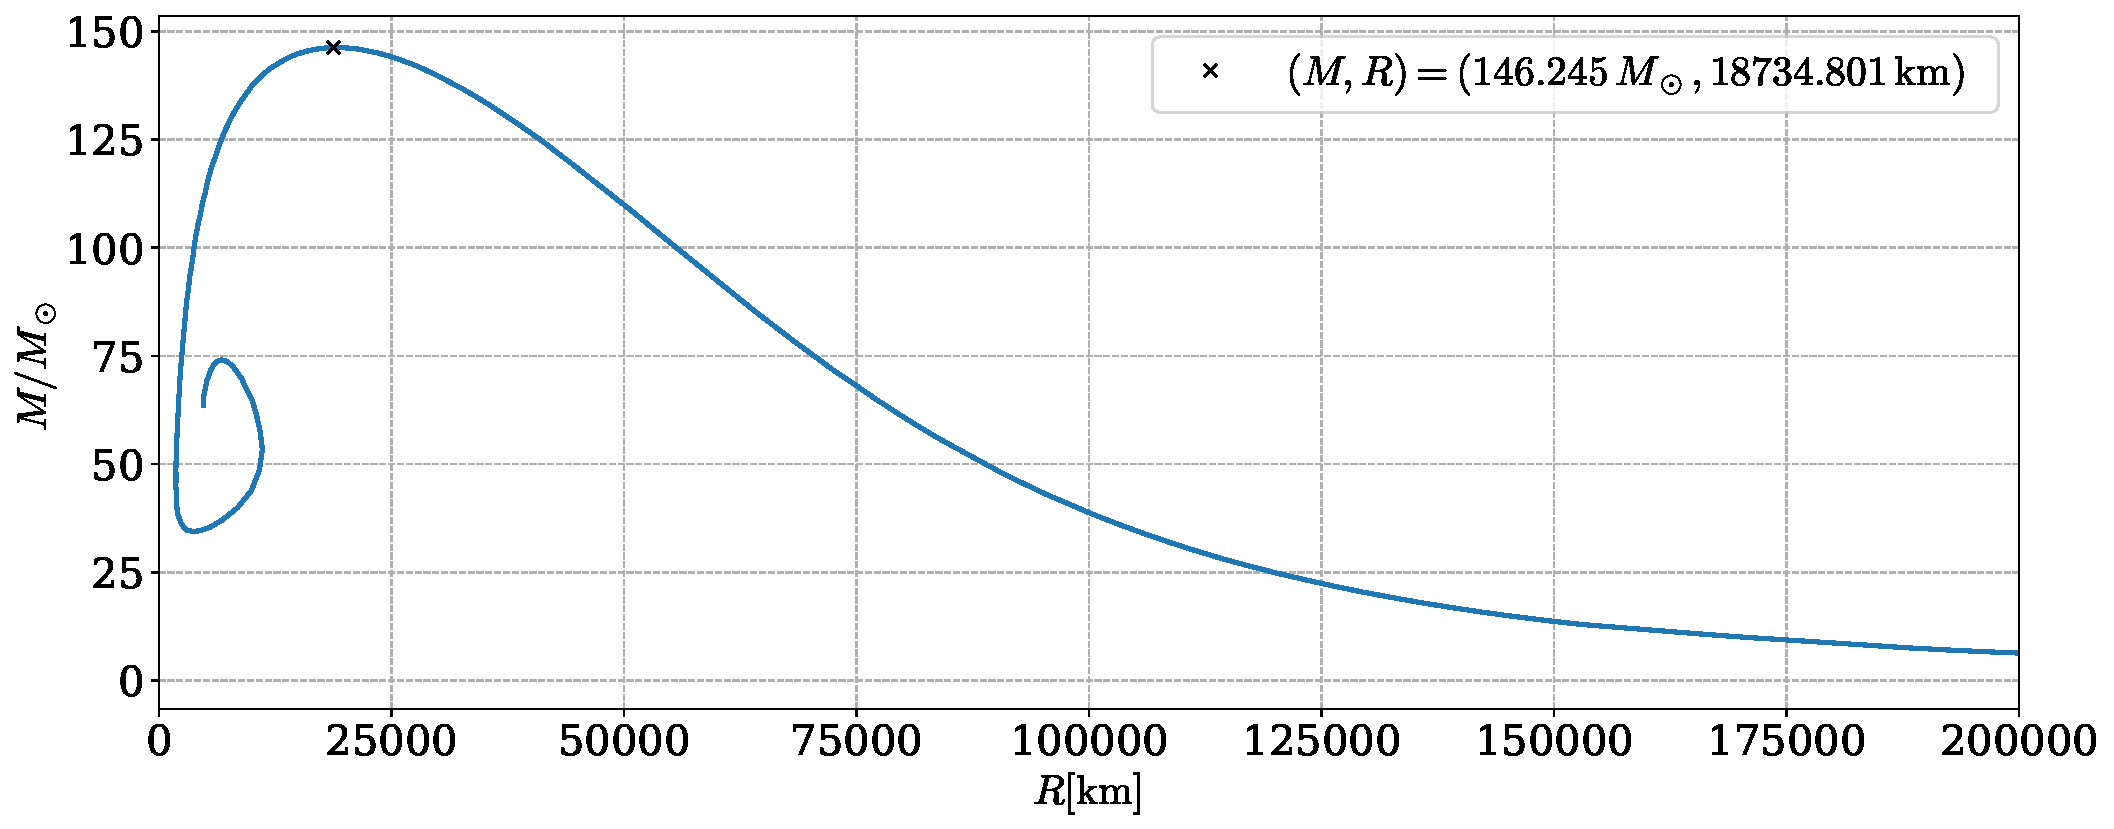
\includegraphics[width=\textwidth]{../scripts/figurer/pion_star/mass_radius__e.pdf}
    \caption{
        The mass-radius relation of pion stars with electrons enforcing charge neutrality.
        The radius is given in kilometers and the mass in units of solar masses.
        }
        \label{fig: mass-radius relation with electrons}
\end{figure}

\begin{figure}[!htb]
    \centering
    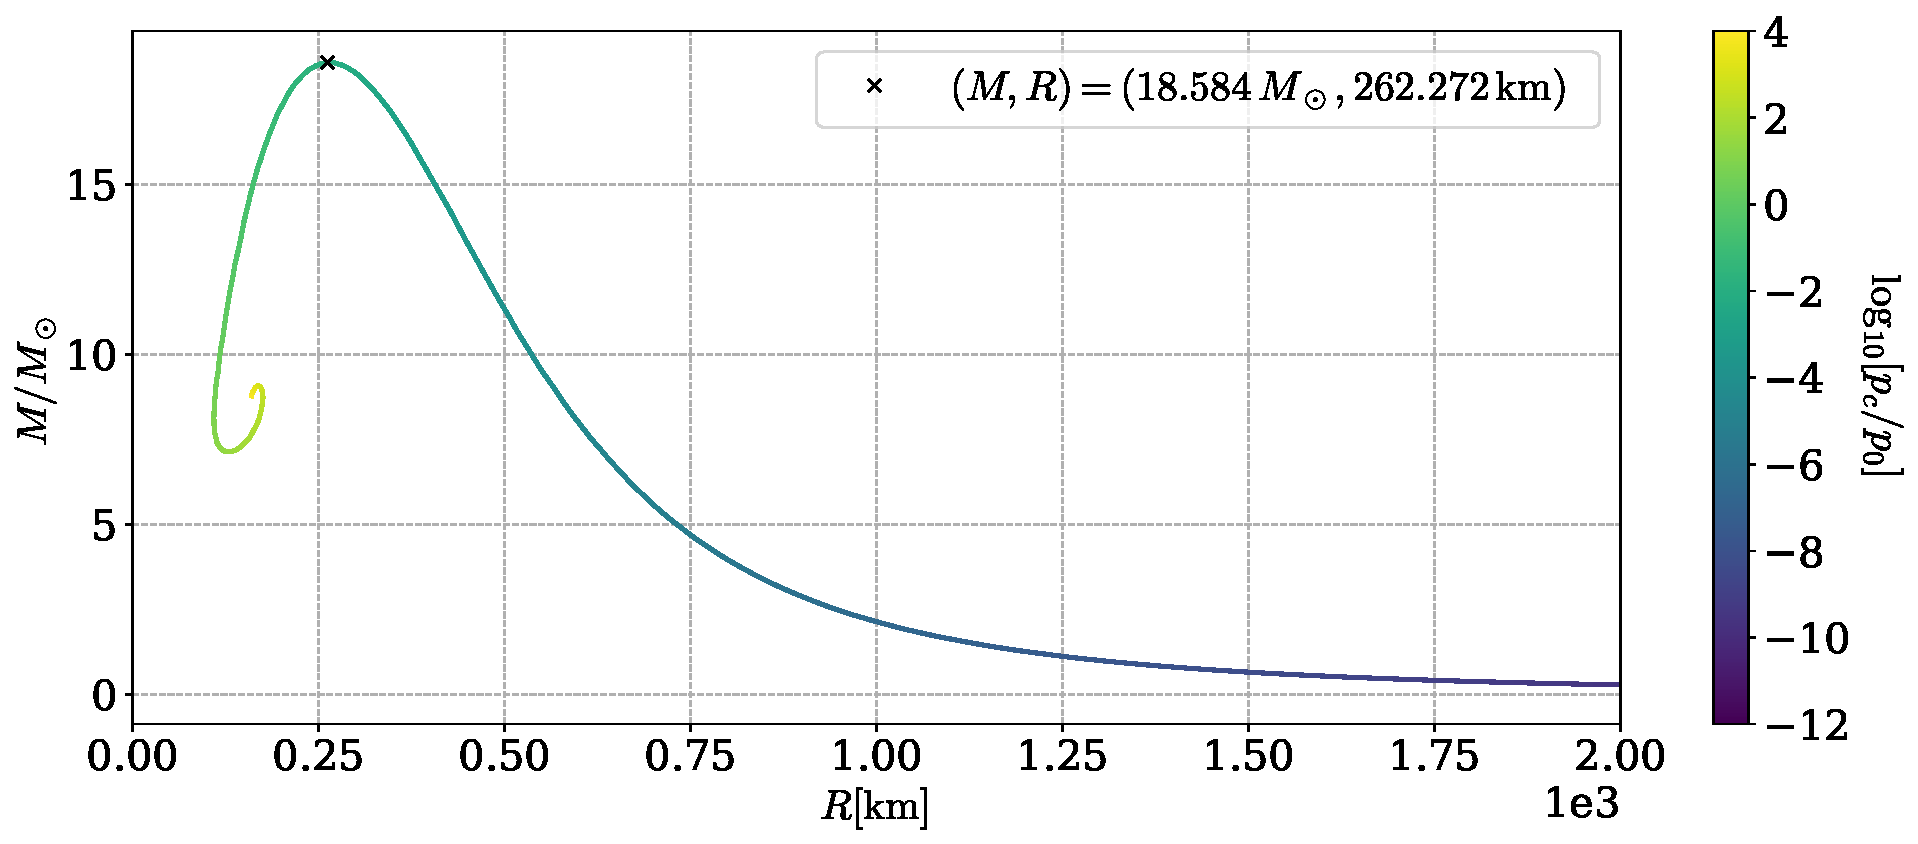
\includegraphics[width=.9\textwidth]{../scripts/figurer/pion_star/mass_radius__mu.pdf}
    \caption{
        The mass-radius relation of pion stars, including leptons to enforce charge neutrality, is compared with pion stars of only pions.
        The radius is given in kilometers and the mass in units of solar masses.
        }
        \label{fig: mass-radius relation with muons}
\end{figure}



\subsection{Neutrinos}

In \autoref{subsection: neutrinos}, we found the equation of state when including neutrinos in addition to charged leptons and the decay of pions due to the weak force.
In this case, the pressure and energy density do not vanish as the isospin density vanishes, but rather as $p = p_\text{min}>0$ as defined in \autoref{p min}
This is due to the contribution of neutrinos.
We therefore define the stellar radius $R$ by $p(R) = p_\text{min}$, where the pion condensate vanishes.
Such a star will therefore have an atmosphere of ultrarelativistic neutrinos.
For $p < p_\text{min}$, the equation of state is that of massless fermions and will therefore not have a finite radius.
There is a $p+u$-term on the right-hand side of the TOV equation, \autoref{TOV}.
When we defined the stellar radius by $p(R) = 0$, this factor vanishes as we approach the surface of the star, while now $p+u \geq 4 p_\text{min}$.
Close to the surface, the pressure will therefore fall faster, as a consequence of $p_\text{min}>0$.
The resulting mass-radius relation is shown in \autoref{fig: mass radius neutrino}.
We see that, in contrast to the earlier results, both the mass and radius approach zero as $p_c \rightarrow p_\text{min}$.


\begin{figure}[!htb]
    \centering
    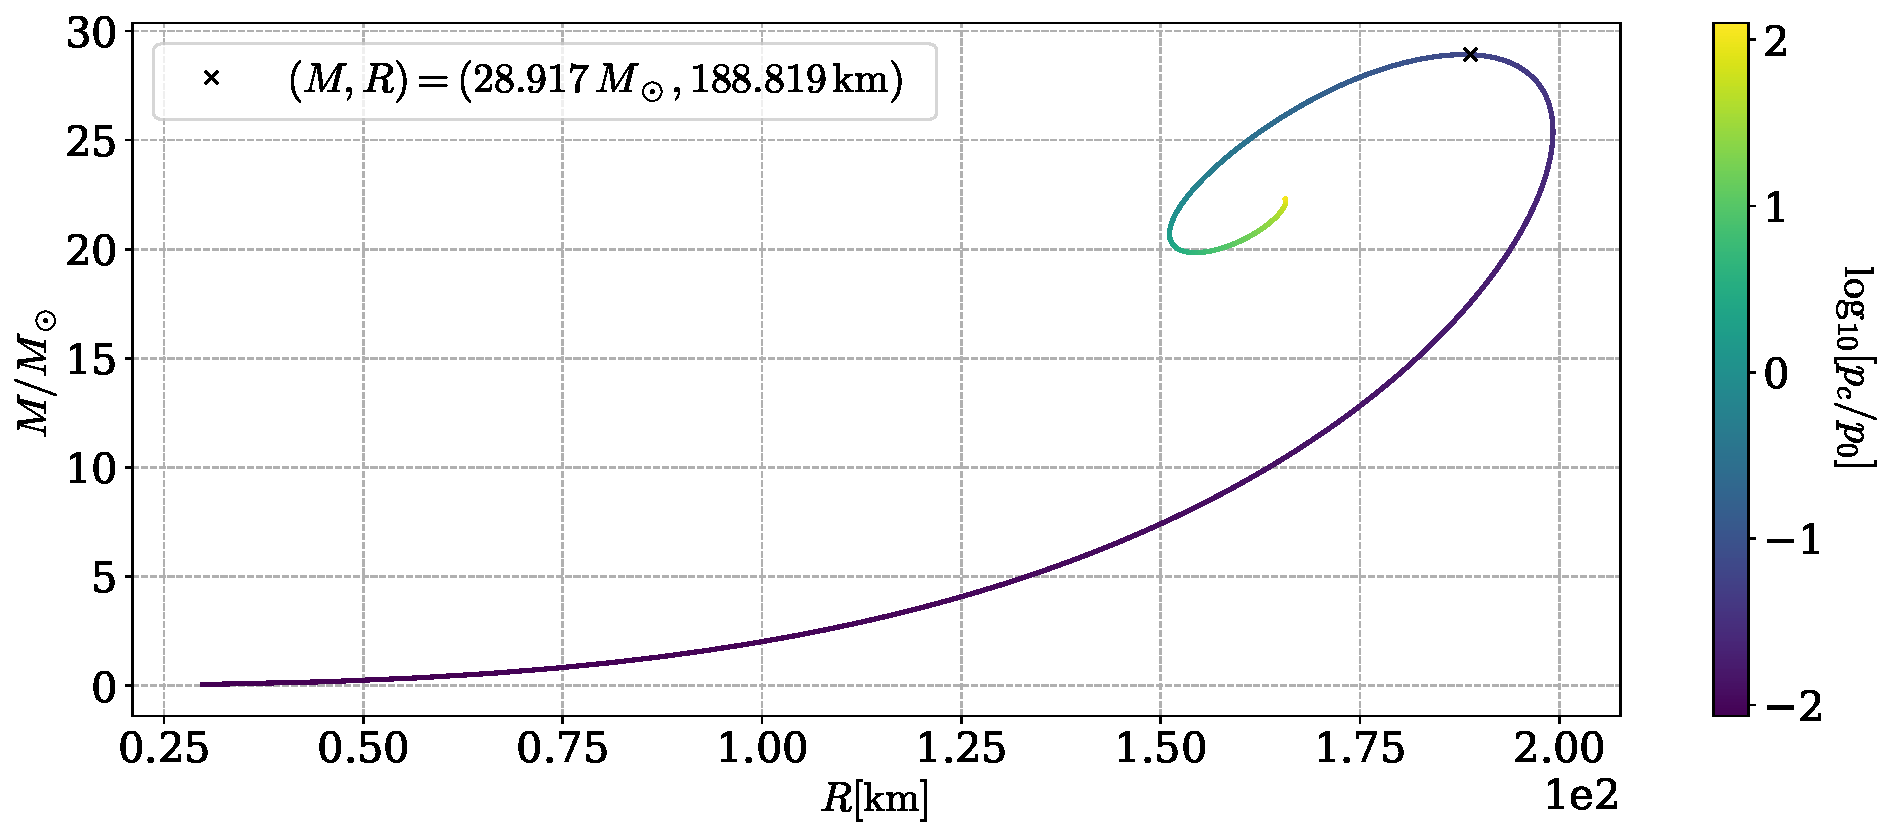
\includegraphics[width=\textwidth]{../scripts/figurer/pion_star/mass_radius_neutrino.pdf}
    \caption{
        The mass-radius relation of pion stars, including leptons and neutrinos in equilibrium.
        The radius is given in kilometers and the mass in units of solar masses.
        }
        \label{fig: mass radius neutrino}
\end{figure}

In \autoref{fig: light stars}, the pion stars including charged leptons and neutrinos are compared to a family of stars with $u = 3p$ but different values for $p_\text{min}$.
We see that the mass-radius relation of the pion star closely resembles that of such a star and that the mass-radius relationship, therefore, is mostly set by $p_\text{min}$.


\begin{figure}[!htb]
    \centering
    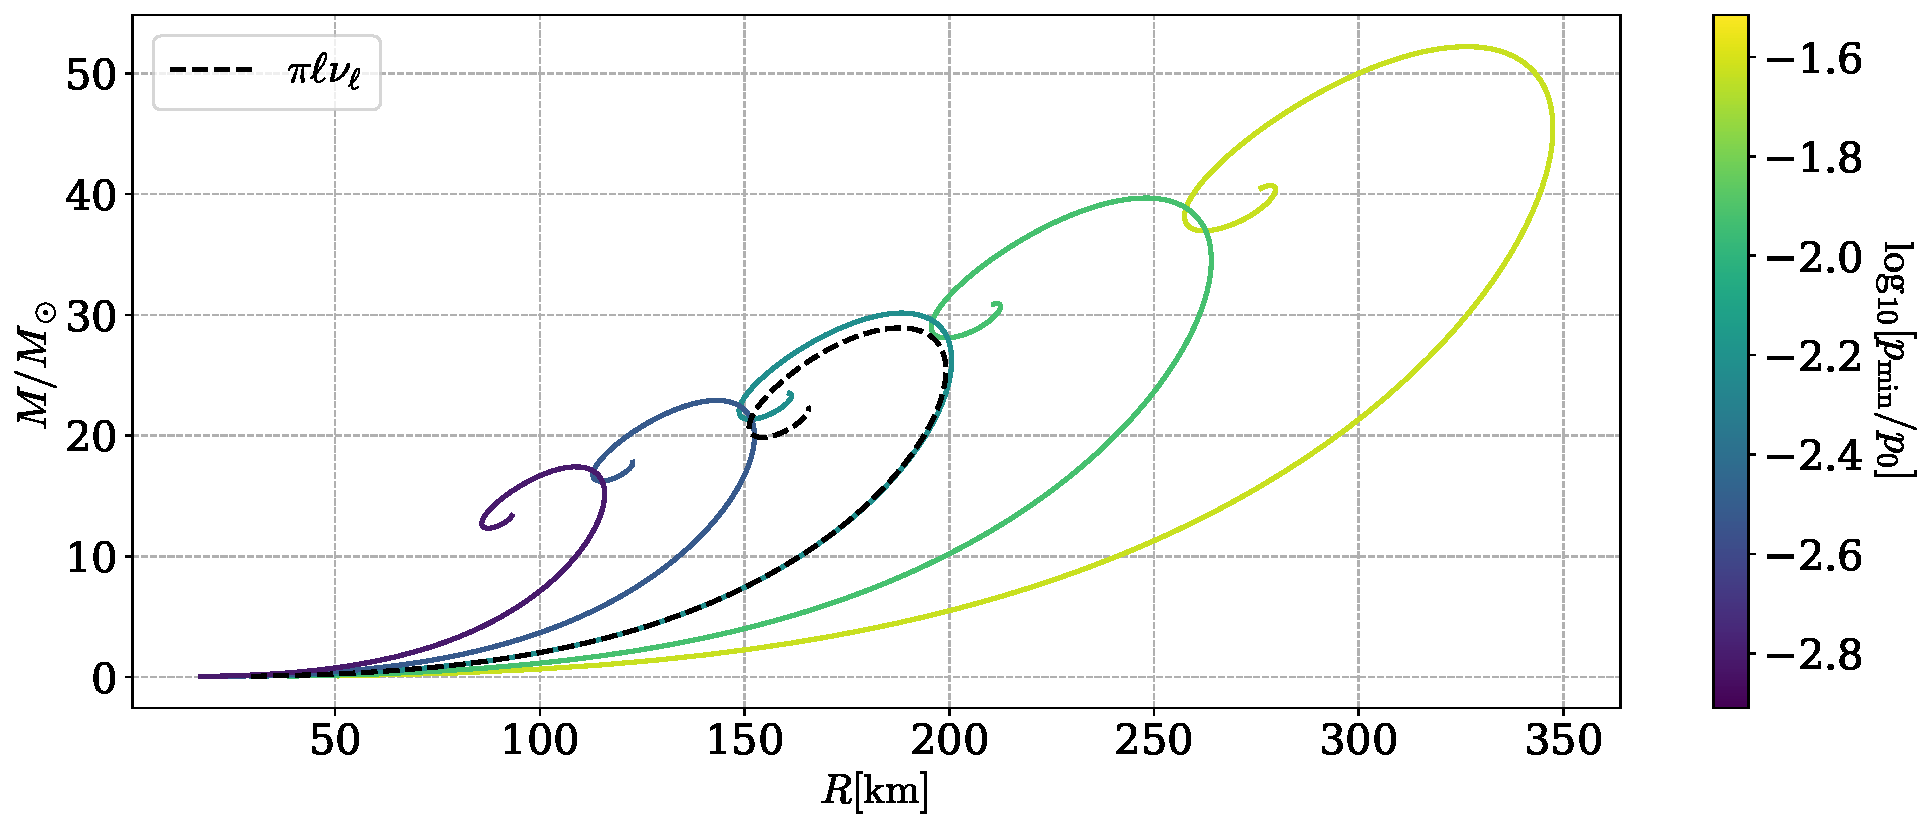
\includegraphics[width=\textwidth]{../scripts/figurer/pion_star/mass_radius_light.pdf}
    \caption{Stars with equation of state $u = 3p$ but different values for $p_\text{min}>0$ is compared to the pion star with charged leptons and neutrinos.}
    \label{fig: light stars}
\end{figure}


\subsection{NLO pion star}

We now use the next-to-leading order results for the pure pion condensate, which we found in \autoref{section: nlo thermodynamics}.
The mass-radius relationship, in this case, is shown in \autoref{fig: mass-radius relation nlo}.
The maximum mass is $M_\text{max} = 9.94\, M_0$, and the corresponding radius is $R = 54.09\,\text{km}$.
In \autoref{fig: mass-radius relation compare nlo}, we compare the leading order and next-to-leading order mass-radius relations.
The results are similar, however, the next-to-leading order star is smaller and less massive, as is expected for a less stiff equation of state.

\begin{figure}[!htb]
    \centering
    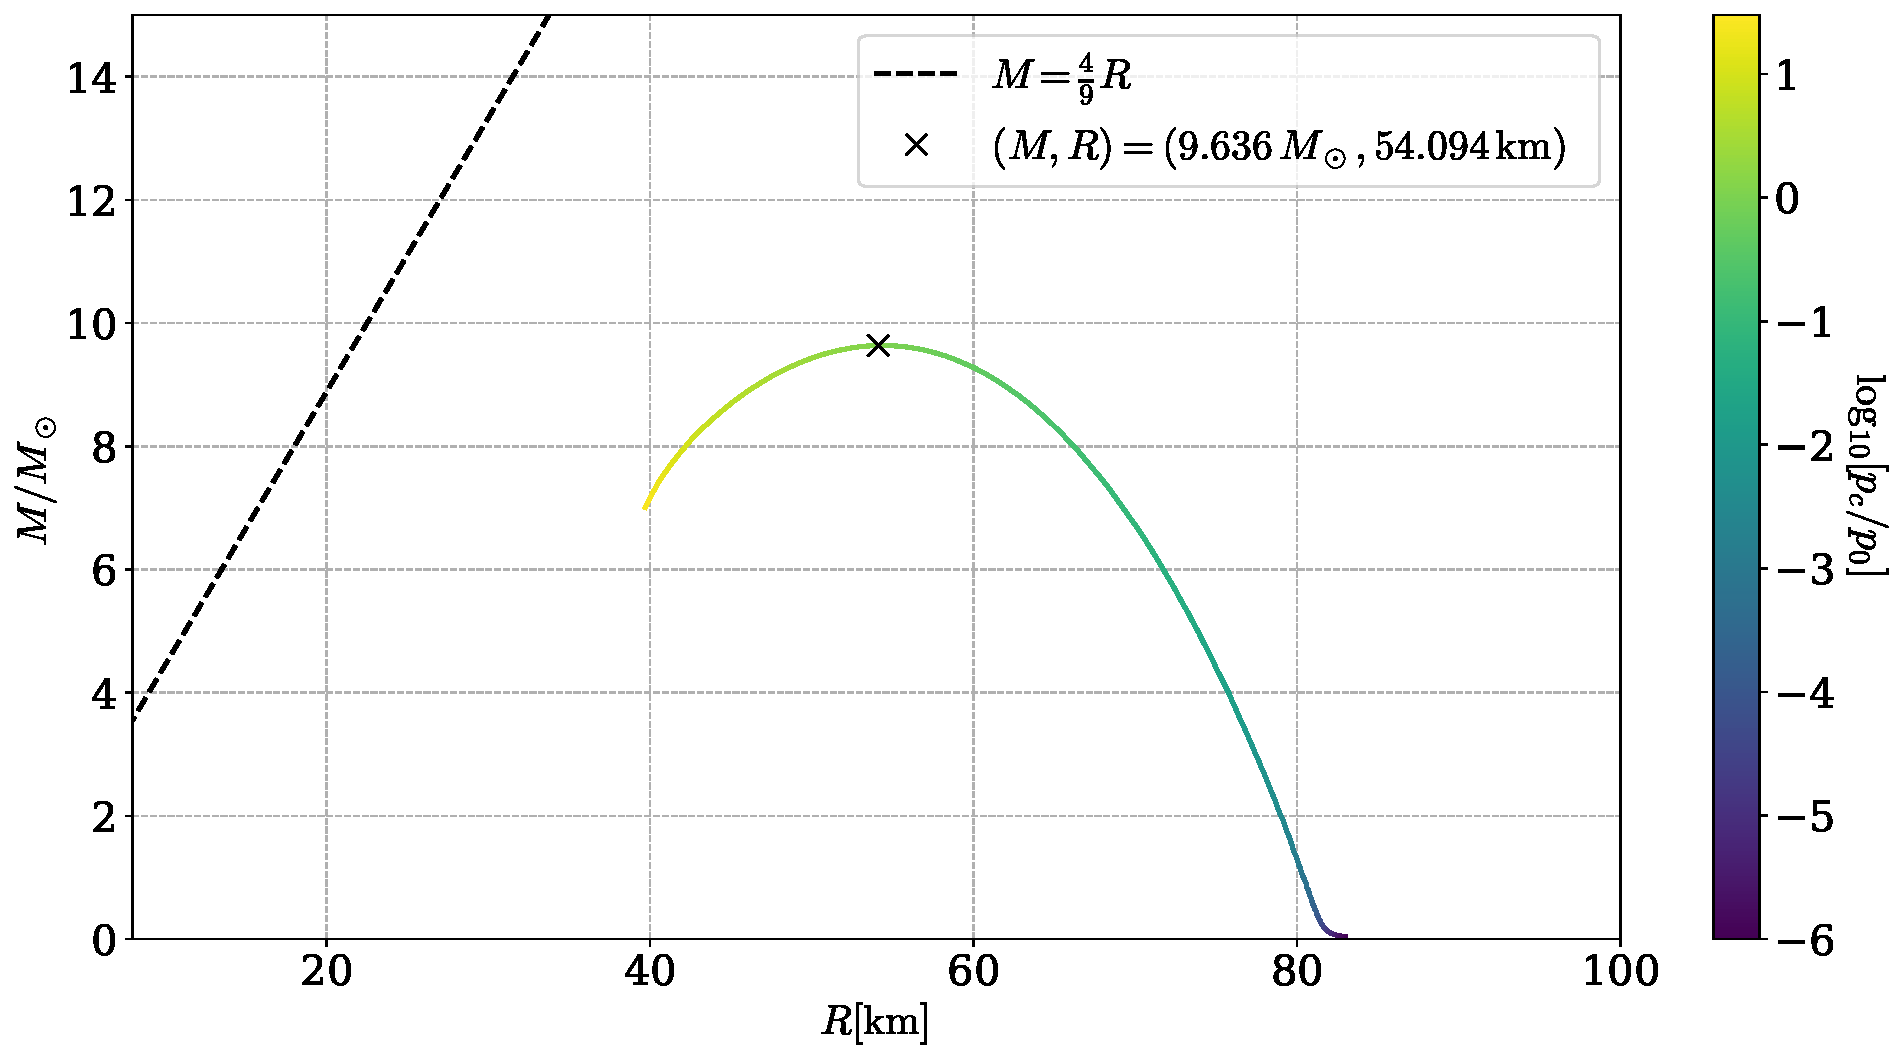
\includegraphics[width=\textwidth]{../scripts/figurer/pion_star/mass_radius_pion_star_nlo.pdf}
    \caption{The mass-radius relation of a pion star with the next-to-leading order equation of state.}
    \label{fig: mass-radius relation nlo}
\end{figure}

\begin{figure}[!htb]
    \centering
    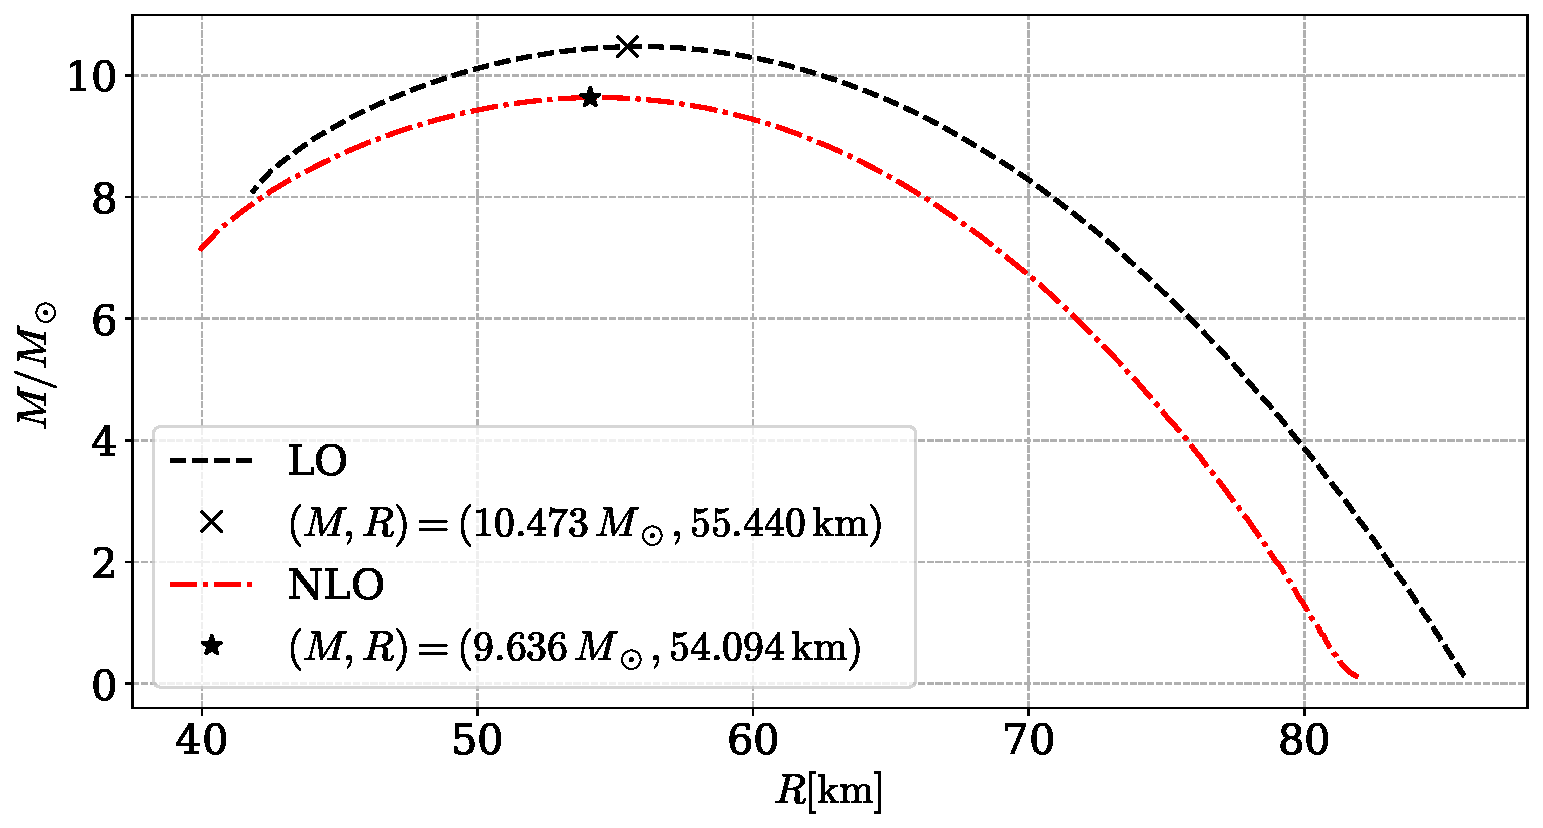
\includegraphics[width=\textwidth]{../scripts/figurer/pion_star/mass_compare_order.pdf}
    \caption{
        The mass-radius relation of a pion star using the leading and next-to-leading order equation of state is compared. 
        The mass is given in solar masses and the radius in kilometers.}
    \label{fig: mass-radius relation compare nlo}
\end{figure}



\section{Comparison and key values}


The various compositions of the pion stars create objects of different characteristics and wildly different sizes.
In \autoref{fig: mass-radius relation with leptons}, we compare the mass-radius of the different stars.
We only include the next-to-leading order result for pure pion condensation, to make the plot more orderly.


\begin{figure}[!htb]
    \centering
    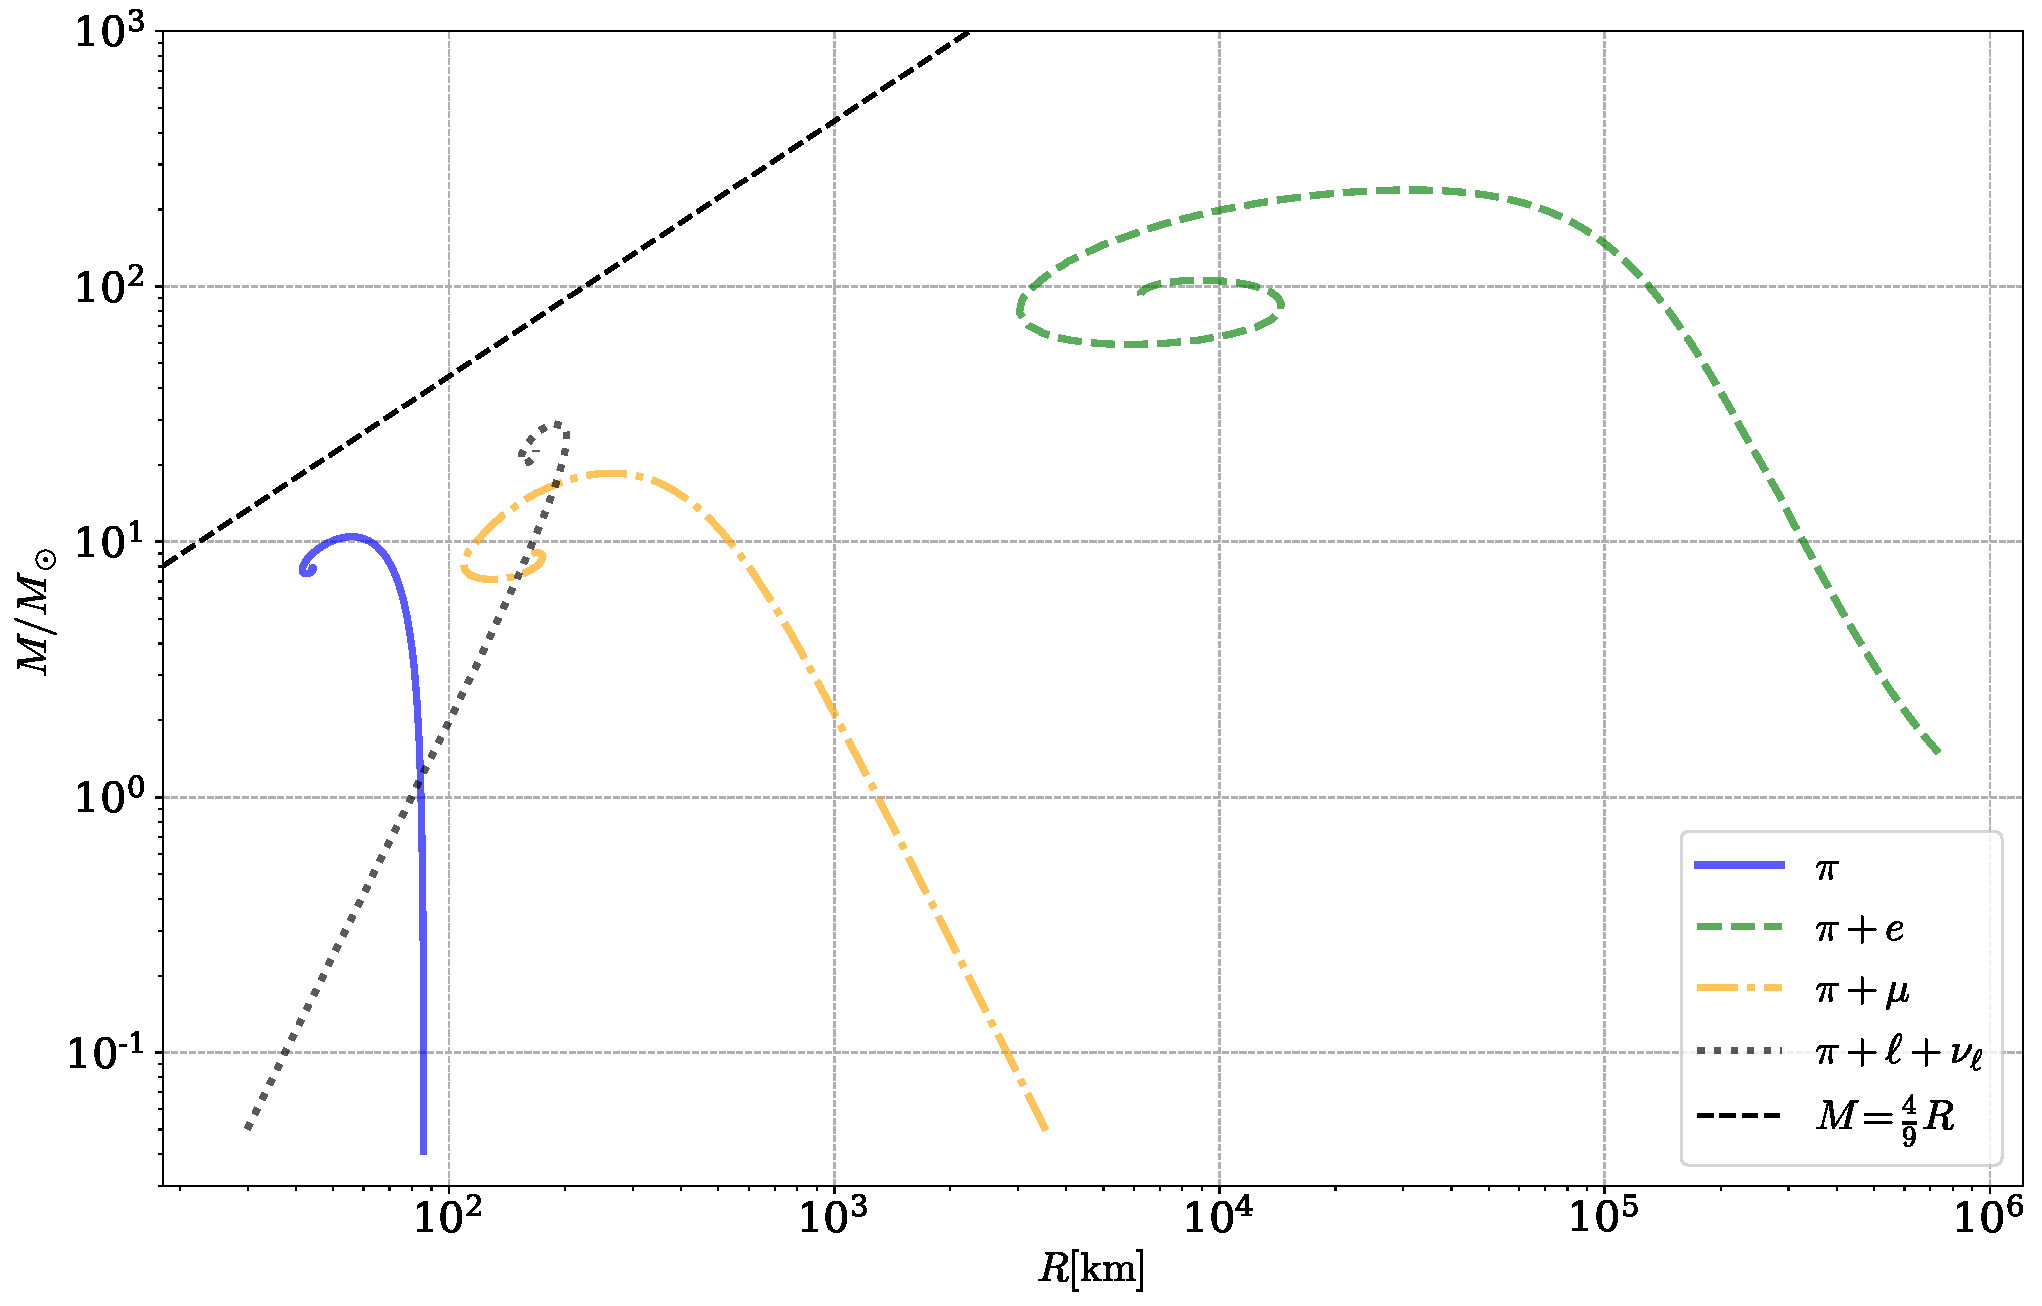
\includegraphics[width=.9\textwidth]{../scripts/figurer/pion_star/mass_radius_all.pdf}
    \caption{
        The mass-radius relation of pion stars, including leptons to enforce charge neutrality, is compared with pion stars of only pions.
        The radius is given in kilometers and the mass in units of solar masses.
        }
        \label{fig: mass-radius relation with leptons}
\end{figure}

\begin{figure}[!htb]
    \centering
    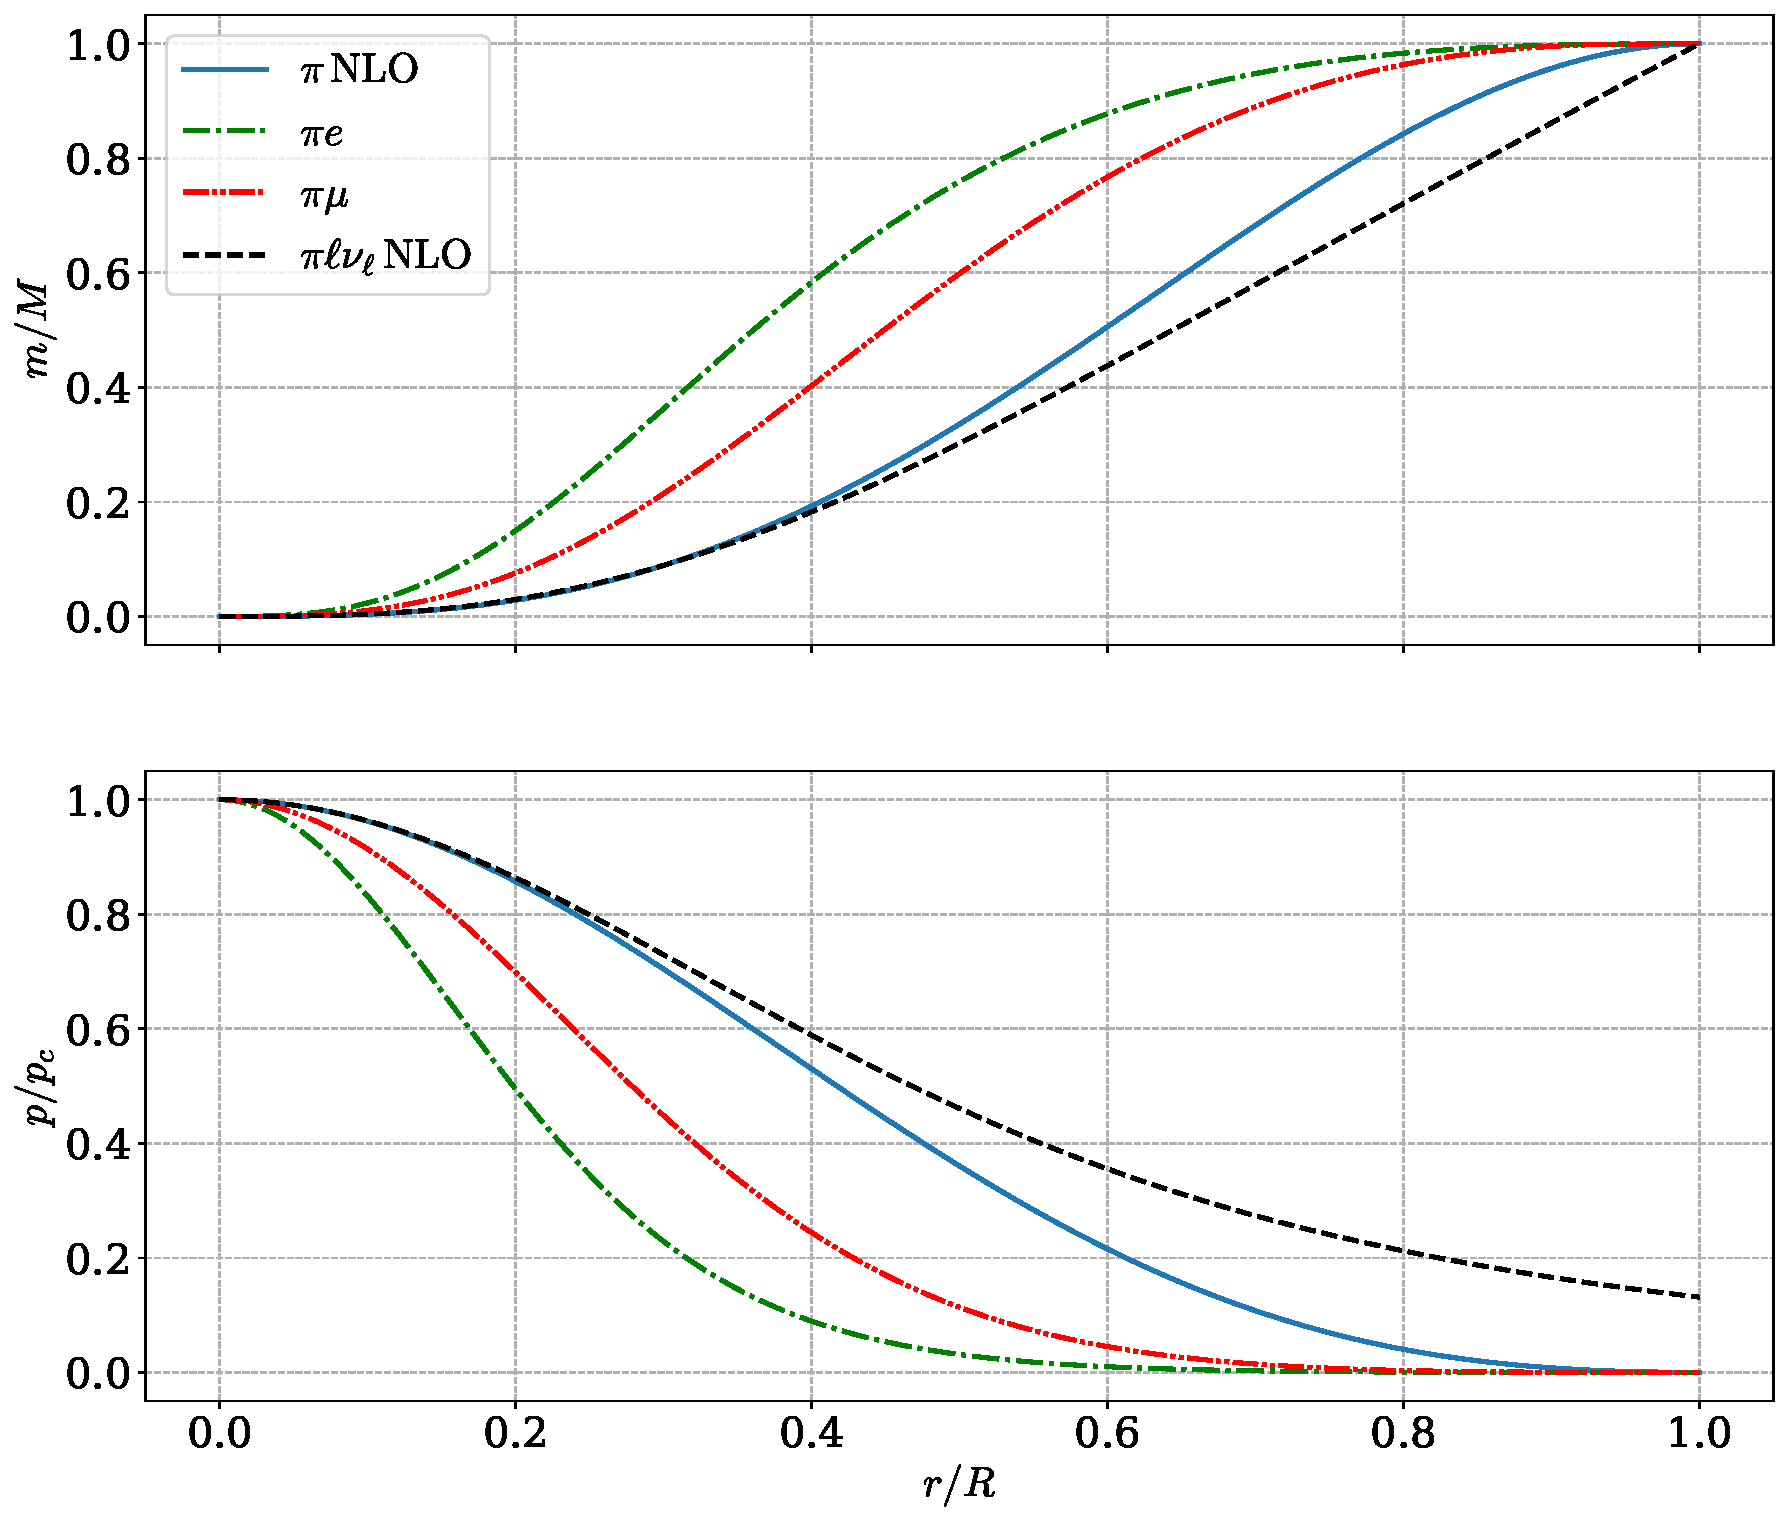
\includegraphics[width=.8\textwidth]{../scripts/figurer/pion_star/max_pressure_mass.pdf}
    \caption{
        The pressure and mass of the maximum-mass configuration of pion stars of various configurations.
        The mass, pressure, and radius are normalized to the star's stellar mass, central pressure and stellar radius.
        }
        \label{fig: max pressure and mass}
\end{figure}


Key values for each system are shown in \autoref{table: key values}.


\begin{table}[!htb]
    \centering
    \caption{The values of various quantities for the maximum mass stars}
    \label{table: key values}
    \begin{tabular}{c  c  c  c  c c c}
        \hline \hline
        system & $M_\text{max}/M_\odot$ & $R / \text{km}$ & 
        $u/u_0$ & $p/u_0$ & $\mu_I/m_\pi-1$ & $\mu_\ell/m_\ell-1$ \\
        \hline
        $\pi\,\, \text{LO}$& 10.47 & 55.38 & 2.864 & 1.318 & 0.8461& \\
        $\pi\, \text{NLO}$& 9.04 & 54.09 & 3.020 & 1.139 & 0.9256 & \\
        $\pi\,\,\text{EM}$& 10.11 & 53.58 & 2.930 & 1.318 & 0.8463 & \\
        $\pi + e$& 283.8 & 3.171$\times10^4$ & 
        2.550$\times10^{-6}$ & 1.995$\times10^{-8}$ & 
        6.222$\times10^{-6}$ & \\
        $\pi + \mu$& 18.58 & 262.3 & 
        0.1411 & 1.202$\times 10^{-2}$ &
        1.732$\times10^{-2}$& \\
        $\pi + \ell + \nu_\ell$& 28.92 & 188.8 &
        0.2262  & 6.847$\times 10^{-2}$ &
        5.264$\times10^{-3}$& \\
        \hline
    \end{tabular}
\end{table}



\section{Comparison with QCD-lattice results}

Results for the equation of state of the pion condensate, as well as the system with pions and electrons or muons, were obtained by \citeauthor{brandtNewClassCompact2018} in \autocite{brandtNewClassCompact2018} using computational QCD lattice methods.
Their results are shown in \autoref{fig: brandt eos} and compared with our results.
There is a good agreement between the results, although the computational results tend to give a slightly less stiff equation of state.

\begin{figure}[!htb]
    \centering
    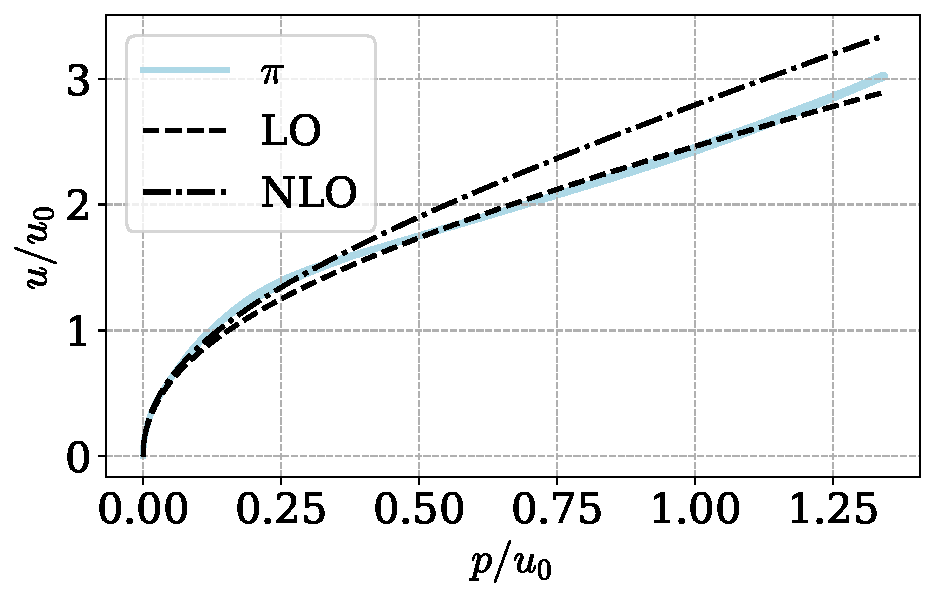
\includegraphics[width=\textwidth]{../scripts/figurer/brandt_eos.pdf}
    \caption{
        The equation of state of only pions, pions and electrons, and pions and muons.
        The results of \citeauthor{brandtNewClassCompact2018}, solid color, are compared with our results, dashed lines.
        The result of \citeauthor{brandtNewClassCompact2018} incorporate statistical and systematic uncertainty in both $u$ and $p$ in the width of the lines.
        Both energy density and pressure are shown in units of $u_0 = f_\pi^2 m_\pi^2$.
    }
    \label{fig: brandt eos}
\end{figure}


With these equations of state, they obtained the mass-radius relations of pion stars.
Their results are compared with ours in  \autoref{fig: brandt mass-radius}.


\begin{figure}[!htb]
    \centering
    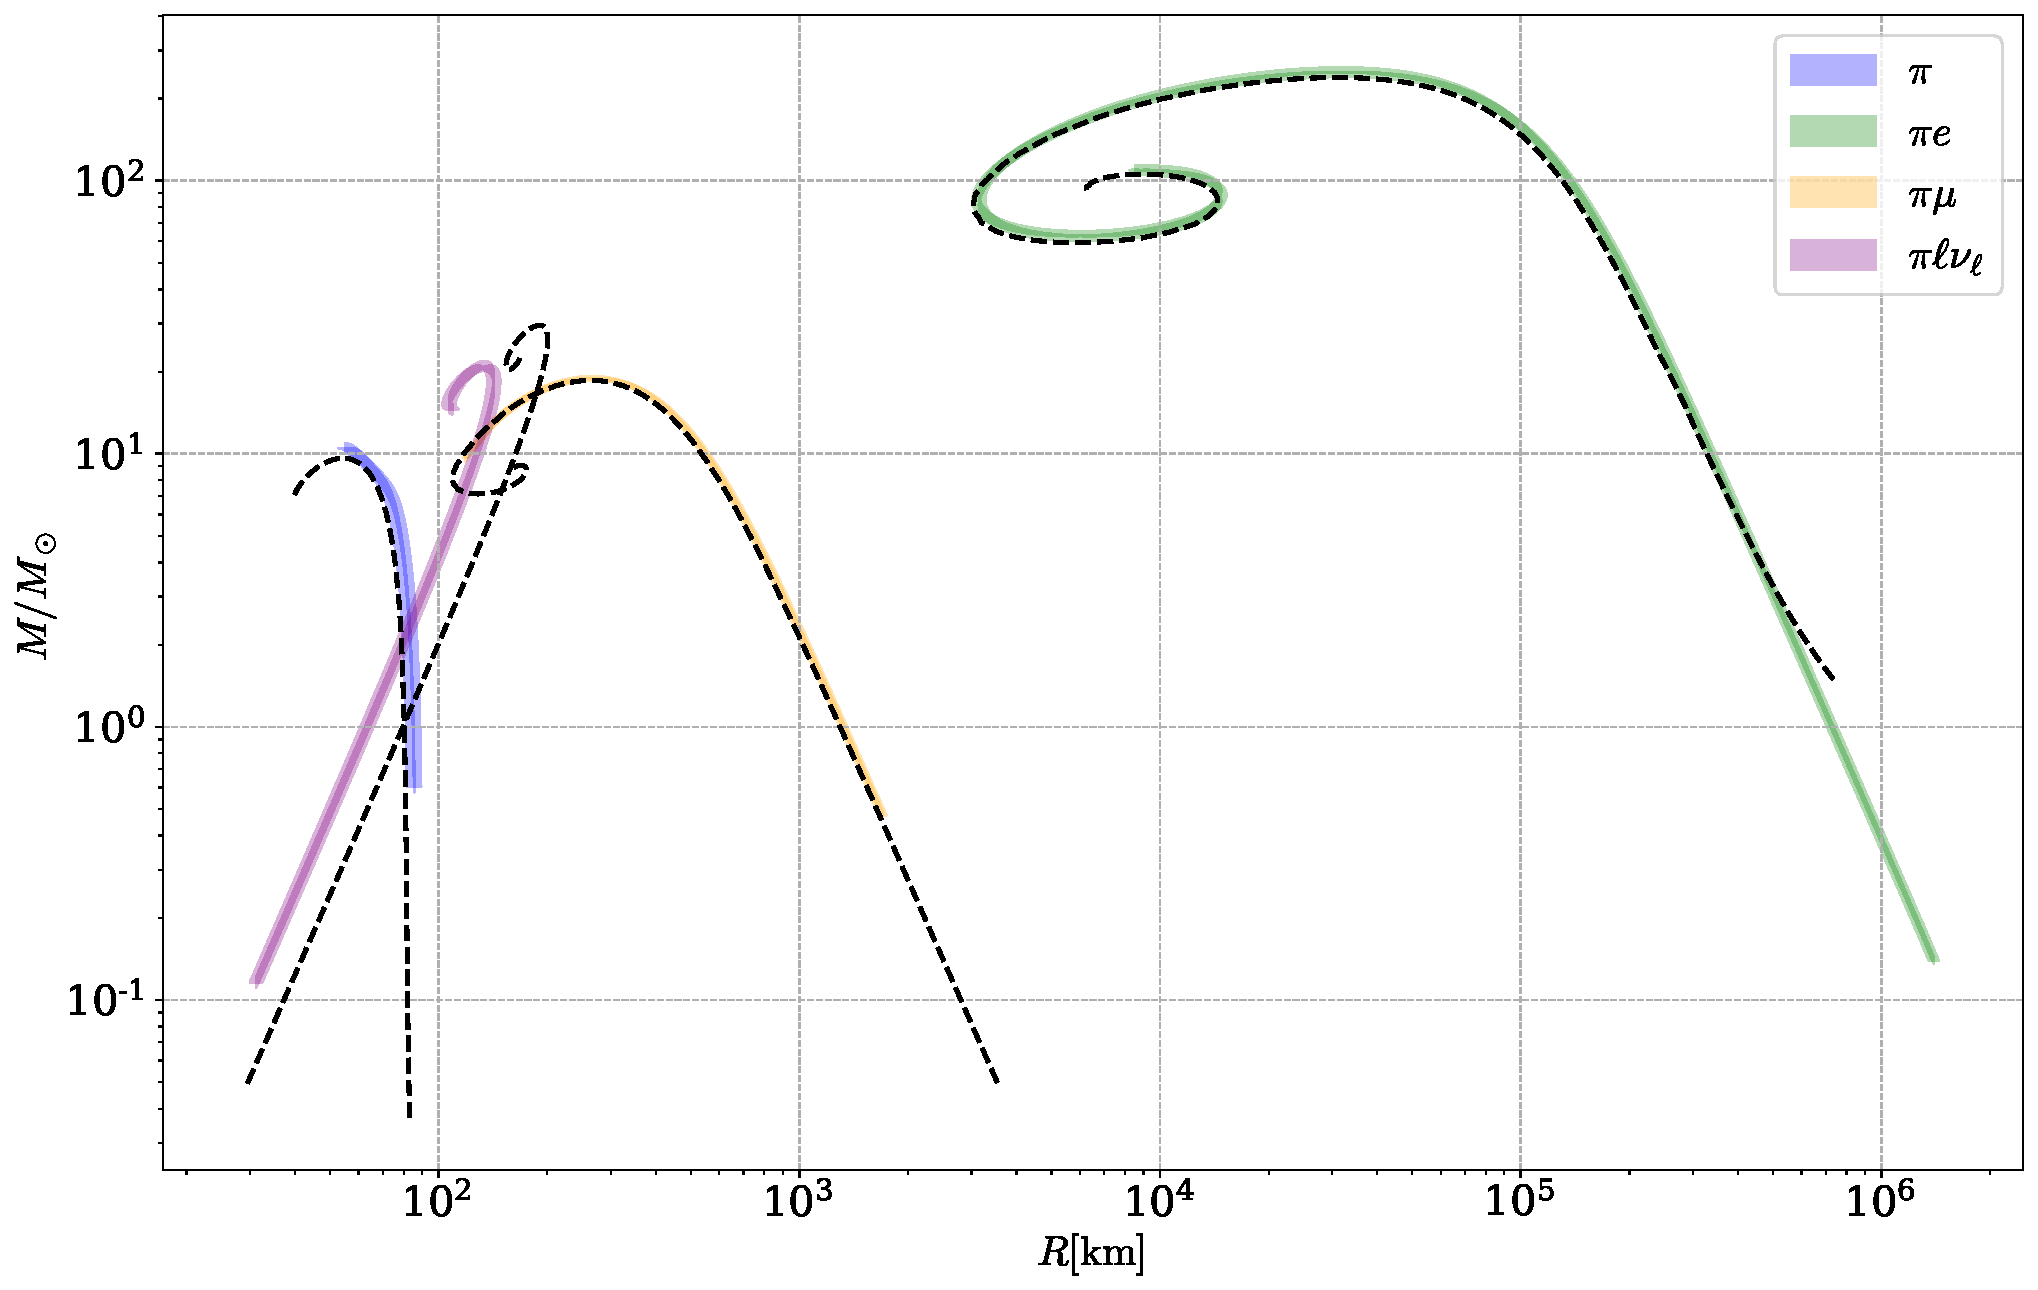
\includegraphics[width=\textwidth]{../scripts/figurer/pion_star/mass_radius_brandt_all.pdf}
    \caption{
        The mass-radius relations for pion stars, with and without leptons included.
        The results of \citeauthor{brandtNewClassCompact2018}, solid color, are compared with our results, dashed lines.
        The result of \citeauthor{brandtNewClassCompact2018} incorporate statistical and systematic uncertainty in both $R$ and $M$ in the width of the lines.
        The radius is in units of $\text{km}$, while mass is in solar masses, $M_\odot$.
    }
    \label{fig: brandt mass-radius}
\end{figure}

